
%% bare_adv.tex
%% V1.4b
%% 2015/08/26
%% by Michael Shell
%% See: 
%% http://www.michaelshell.org/
%% for current contact information.
%%
%% This is a skeleton file demonstrating the advanced use of IEEEtran.cls
%% (requires IEEEtran.cls version 1.8b or later) with an IEEE Computer
%% Society journal paper.
%%
%% Support sites:
%% http://www.michaelshell.org/tex/ieeetran/
%% http://www.ctan.org/pkg/ieeetran
%% and
%% http://www.ieee.org/

%%*************************************************************************
%% Legal Notice:
%% This code is offered as-is without any warranty either expressed or
%% implied; without even the implied warranty of MERCHANTABILITY or
%% FITNESS FOR A PARTICULAR PURPOSE! 
%% User assumes all risk.
%% In no event shall the IEEE or any contributor to this code be liable for
%% any damages or losses, including, but not limited to, incidental,
%% consequential, or any other damages, resulting from the use or misuse
%% of any information contained here.
%%
%% All comments are the opinions of their respective authors and are not
%% necessarily endorsed by the IEEE.
%%
%% This work is distributed under the LaTeX Project Public License (LPPL)
%% ( http://www.latex-project.org/ ) version 1.3, and may be freely used,
%% distributed and modified. A copy of the LPPL, version 1.3, is included
%% in the base LaTeX documentation of all distributions of LaTeX released
%% 2003/12/01 or later.
%% Retain all contribution notices and credits.
%% ** Modified files should be clearly indicated as such, including  **
%% ** renaming them and changing author support contact information. **
%%*************************************************************************


% *** Authors should verify (and, if needed, correct) their LaTeX system  ***
% *** with the testflow diagnostic prior to trusting their LaTeX platform ***
% *** with production work. The IEEE's font choices and paper sizes can   ***
% *** trigger bugs that do not appear when using other class files.       ***                          ***
% The testflow support page is at:
% http://www.michaelshell.org/tex/testflow/


% IEEEtran V1.7 and later provides for these CLASSINPUT macros to allow the
% user to reprogram some IEEEtran.cls defaults if needed. These settings
% override the internal defaults of IEEEtran.cls regardless of which class
% options are used. Do not use these unless you have good reason to do so as
% they can result in nonIEEE compliant documents. User beware. ;)
%
%\newcommand{\CLASSINPUTbaselinestretch}{1.0} % baselinestretch
%\newcommand{\CLASSINPUTinnersidemargin}{1in} % inner side margin
%\newcommand{\CLASSINPUToutersidemargin}{1in} % outer side margin
%\newcommand{\CLASSINPUTtoptextmargin}{1in}   % top text margin
%\newcommand{\CLASSINPUTbottomtextmargin}{1in}% bottom text margin




%
\documentclass[10pt,journal,compsoc]{IEEEtran}
% If IEEEtran.cls has not been installed into the LaTeX system files,
% manually specify the path to it like:
% \documentclass[10pt,journal,compsoc]{../sty/IEEEtran}


% For Computer Society journals, IEEEtran defaults to the use of 
% Palatino/Palladio as is done in IEEE Computer Society journals.
% To go back to Times Roman, you can use this code:
%\renewcommand{\rmdefault}{ptm}\selectfont





% Some very useful LaTeX packages include:
% (uncomment the ones you want to load)



% *** MISC UTILITY PACKAGES ***
%
%\usepackage{ifpdf}
% Heiko Oberdiek's ifpdf.sty is very useful if you need conditional
% compilation based on whether the output is pdf or dvi.
% usage:
% \ifpdf
%   % pdf code
% \else
%   % dvi code
% \fi
% The latest version of ifpdf.sty can be obtained from:
% http://www.ctan.org/pkg/ifpdf
% Also, note that IEEEtran.cls V1.7 and later provides a builtin
% \ifCLASSINFOpdf conditional that works the same way.
% When switching from latex to pdflatex and vice-versa, the compiler may
% have to be run twice to clear warning/error messages.






% *** CITATION PACKAGES ***
%
\ifCLASSOPTIONcompsoc
  % The IEEE Computer Society needs nocompress option
  % requires cite.sty v4.0 or later (November 2003)
  \usepackage[nocompress]{cite}
\else
  % normal IEEE
  \usepackage{cite}
\fi
\usepackage{array}
\usepackage{graphicx}
\usepackage{multirow}
\usepackage{caption}
\usepackage{tabularx, booktabs}
\newcolumntype{C}{>{\centering\arraybackslash}X} % centered version of "X" type
% cite.sty was written by Donald Arseneau
% V1.6 and later of IEEEtran pre-defines the format of the cite.sty package
% \cite{} output to follow that of the IEEE. Loading the cite package will
% result in citation numbers being automatically sorted and properly
% "compressed/ranged". e.g., [1], [9], [2], [7], [5], [6] without using
% cite.sty will become [1], [2], [5]--[7], [9] using cite.sty. cite.sty's
% \cite will automatically add leading space, if needed. Use cite.sty's
% noadjust option (cite.sty V3.8 and later) if you want to turn this off
% such as if a citation ever needs to be enclosed in parenthesis.
% cite.sty is already installed on most LaTeX systems. Be sure and use
% version 5.0 (2009-03-20) and later if using hyperref.sty.
% The latest version can be obtained at:
% http://www.ctan.org/pkg/cite
% The documentation is contained in the cite.sty file itself.
%
% Note that some packages require special options to format as the Computer
% Society requires. In particular, Computer Society  papers do not use
% compressed citation ranges as is done in typical IEEE papers
% (e.g., [1]-[4]). Instead, they list every citation separately in order
% (e.g., [1], [2], [3], [4]). To get the latter we need to load the cite
% package with the nocompress option which is supported by cite.sty v4.0
% and later.





% *** GRAPHICS RELATED PACKAGES ***
%
\ifCLASSINFOpdf
  % \usepackage[pdftex]{graphicx}
  % declare the path(s) where your graphic files are
  % \graphicspath{{../pdf/}{../jpeg/}}
  % and their extensions so you won't have to specify these with
  % every instance of \includegraphics
  % \DeclareGraphicsExtensions{.pdf,.jpeg,.png}
\else
  % or other class option (dvipsone, dvipdf, if not using dvips). graphicx
  % will default to the driver specified in the system graphics.cfg if no
  % driver is specified.
  % \usepackage[dvips]{graphicx}
  % declare the path(s) where your graphic files are
  % \graphicspath{{../eps/}}
  % and their extensions so you won't have to specify these with
  % every instance of \includegraphics
  % \DeclareGraphicsExtensions{.eps}
\fi
% graphicx was written by David Carlisle and Sebastian Rahtz. It is
% required if you want graphics, photos, etc. graphicx.sty is already
% installed on most LaTeX systems. The latest version and documentation
% can be obtained at: 
% http://www.ctan.org/pkg/graphicx
% Another good source of documentation is "Using Imported Graphics in
% LaTeX2e" by Keith Reckdahl which can be found at:
% http://www.ctan.org/pkg/epslatex
%
% latex, and pdflatex in dvi mode, support graphics in encapsulated
% postscript (.eps) format. pdflatex in pdf mode supports graphics
% in .pdf, .jpeg, .png and .mps (metapost) formats. Users should ensure
% that all non-photo figures use a vector format (.eps, .pdf, .mps) and
% not a bitmapped formats (.jpeg, .png). The IEEE frowns on bitmapped formats
% which can result in "jaggedy"/blurry rendering of lines and letters as
% well as large increases in file sizes.
%
% You can find documentation about the pdfTeX application at:
% http://www.tug.org/applications/pdftex





% *** MATH PACKAGES ***
%
%\usepackage{amsmath}
% A popular package from the American Mathematical Society that provides
% many useful and powerful commands for dealing with mathematics.
%
% Note that the amsmath package sets \interdisplaylinepenalty to 10000
% thus preventing page breaks from occurring within multiline equations. Use:
%\interdisplaylinepenalty=2500
% after loading amsmath to restore such page breaks as IEEEtran.cls normally
% does. amsmath.sty is already installed on most LaTeX systems. The latest
% version and documentation can be obtained at:
% http://www.ctan.org/pkg/amsmath





% *** SPECIALIZED LIST PACKAGES ***
%\usepackage{acronym}
% acronym.sty was written by Tobias Oetiker. This package provides tools for
% managing documents with large numbers of acronyms. (You don't *have* to
% use this package - unless you have a lot of acronyms, you may feel that
% such package management of them is bit of an overkill.)
% Do note that the acronym environment (which lists acronyms) will have a
% problem when used under IEEEtran.cls because acronym.sty relies on the
% description list environment - which IEEEtran.cls has customized for
% producing IEEE style lists. A workaround is to declared the longest
% label width via the IEEEtran.cls \IEEEiedlistdecl global control:
%
% \renewcommand{\IEEEiedlistdecl}{\IEEEsetlabelwidth{SONET}}
% \begin{acronym}
%
% \end{acronym}
% \renewcommand{\IEEEiedlistdecl}{\relax}% remember to reset \IEEEiedlistdecl
%
% instead of using the acronym environment's optional argument.
% The latest version and documentation can be obtained at:
% http://www.ctan.org/pkg/acronym


%\usepackage{algorithmic}
% algorithmic.sty was written by Peter Williams and Rogerio Brito.
% This package provides an algorithmic environment fo describing algorithms.
% You can use the algorithmic environment in-text or within a figure
% environment to provide for a floating algorithm. Do NOT use the algorithm
% floating environment provided by algorithm.sty (by the same authors) or
% algorithm2e.sty (by Christophe Fiorio) as the IEEE does not use dedicated
% algorithm float types and packages that provide these will not provide
% correct IEEE style captions. The latest version and documentation of
% algorithmic.sty can be obtained at:
% http://www.ctan.org/pkg/algorithms
% Also of interest may be the (relatively newer and more customizable)
% algorithmicx.sty package by Szasz Janos:
% http://www.ctan.org/pkg/algorithmicx




% *** ALIGNMENT PACKAGES ***
%
%\usepackage{array}
% Frank Mittelbach's and David Carlisle's array.sty patches and improves
% the standard LaTeX2e array and tabular environments to provide better
% appearance and additional user controls. As the default LaTeX2e table
% generation code is lacking to the point of almost being broken with
% respect to the quality of the end results, all users are strongly
% advised to use an enhanced (at the very least that provided by array.sty)
% set of table tools. array.sty is already installed on most systems. The
% latest version and documentation can be obtained at:
% http://www.ctan.org/pkg/array


%\usepackage{mdwmath}
%\usepackage{mdwtab}
% Also highly recommended is Mark Wooding's extremely powerful MDW tools,
% especially mdwmath.sty and mdwtab.sty which are used to format equations
% and tables, respectively. The MDWtools set is already installed on most
% LaTeX systems. The lastest version and documentation is available at:
% http://www.ctan.org/pkg/mdwtools


% IEEEtran contains the IEEEeqnarray family of commands that can be used to
% generate multiline equations as well as matrices, tables, etc., of high
% quality.


%\usepackage{eqparbox}
% Also of notable interest is Scott Pakin's eqparbox package for creating
% (automatically sized) equal width boxes - aka "natural width parboxes".
% Available at:
% http://www.ctan.org/pkg/eqparbox




% *** SUBFIGURE PACKAGES ***
%\ifCLASSOPTIONcompsoc
%  \usepackage[caption=false,font=footnotesize,labelfont=sf,textfont=sf]{subfig}
%\else
%  \usepackage[caption=false,font=footnotesize]{subfig}
%\fi
% subfig.sty, written by Steven Douglas Cochran, is the modern replacement
% for subfigure.sty, the latter of which is no longer maintained and is
% incompatible with some LaTeX packages including fixltx2e. However,
% subfig.sty requires and automatically loads Axel Sommerfeldt's caption.sty
% which will override IEEEtran.cls' handling of captions and this will result
% in non-IEEE style figure/table captions. To prevent this problem, be sure
% and invoke subfig.sty's "caption=false" package option (available since
% subfig.sty version 1.3, 2005/06/28) as this is will preserve IEEEtran.cls
% handling of captions.
% Note that the Computer Society format requires a sans serif font rather
% than the serif font used in traditional IEEE formatting and thus the need
% to invoke different subfig.sty package options depending on whether
% compsoc mode has been enabled.
%
% The latest version and documentation of subfig.sty can be obtained at:
% http://www.ctan.org/pkg/subfig




% *** FLOAT PACKAGES ***
%
%\usepackage{fixltx2e}
% fixltx2e, the successor to the earlier fix2col.sty, was written by
% Frank Mittelbach and David Carlisle. This package corrects a few problems
% in the LaTeX2e kernel, the most notable of which is that in current
% LaTeX2e releases, the ordering of single and double column floats is not
% guaranteed to be preserved. Thus, an unpatched LaTeX2e can allow a
% single column figure to be placed prior to an earlier double column
% figure.
% Be aware that LaTeX2e kernels dated 2015 and later have fixltx2e.sty's
% corrections already built into the system in which case a warning will
% be issued if an attempt is made to load fixltx2e.sty as it is no longer
% needed.
% The latest version and documentation can be found at:
% http://www.ctan.org/pkg/fixltx2e


%\usepackage{stfloats}
% stfloats.sty was written by Sigitas Tolusis. This package gives LaTeX2e
% the ability to do double column floats at the bottom of the page as well
% as the top. (e.g., "\begin{figure*}[!b]" is not normally possible in
% LaTeX2e). It also provides a command:
%\fnbelowfloat
% to enable the placement of footnotes below bottom floats (the standard
% LaTeX2e kernel puts them above bottom floats). This is an invasive package
% which rewrites many portions of the LaTeX2e float routines. It may not work
% with other packages that modify the LaTeX2e float routines. The latest
% version and documentation can be obtained at:
% http://www.ctan.org/pkg/stfloats
% Do not use the stfloats baselinefloat ability as the IEEE does not allow
% \baselineskip to stretch. Authors submitting work to the IEEE should note
% that the IEEE rarely uses double column equations and that authors should try
% to avoid such use. Do not be tempted to use the cuted.sty or midfloat.sty
% packages (also by Sigitas Tolusis) as the IEEE does not format its papers in
% such ways.
% Do not attempt to use stfloats with fixltx2e as they are incompatible.
% Instead, use Morten Hogholm'a dblfloatfix which combines the features
% of both fixltx2e and stfloats:
%
% \usepackage{dblfloatfix}
% The latest version can be found at:
% http://www.ctan.org/pkg/dblfloatfix


%\ifCLASSOPTIONcaptionsoff
%  \usepackage[nomarkers]{endfloat}
% \let\MYoriglatexcaption\caption
% \renewcommand{\caption}[2][\relax]{\MYoriglatexcaption[#2]{#2}}
%\fi
% endfloat.sty was written by James Darrell McCauley, Jeff Goldberg and 
% Axel Sommerfeldt. This package may be useful when used in conjunction with 
% IEEEtran.cls'  captionsoff option. Some IEEE journals/societies require that
% submissions have lists of figures/tables at the end of the paper and that
% figures/tables without any captions are placed on a page by themselves at
% the end of the document. If needed, the draftcls IEEEtran class option or
% \CLASSINPUTbaselinestretch interface can be used to increase the line
% spacing as well. Be sure and use the nomarkers option of endfloat to
% prevent endfloat from "marking" where the figures would have been placed
% in the text. The two hack lines of code above are a slight modification of
% that suggested by in the endfloat docs (section 8.4.1) to ensure that
% the full captions always appear in the list of figures/tables - even if
% the user used the short optional argument of \caption[]{}.
% IEEE papers do not typically make use of \caption[]'s optional argument,
% so this should not be an issue. A similar trick can be used to disable
% captions of packages such as subfig.sty that lack options to turn off
% the subcaptions:
% For subfig.sty:
% \let\MYorigsubfloat\subfloat
% \renewcommand{\subfloat}[2][\relax]{\MYorigsubfloat[]{#2}}
% However, the above trick will not work if both optional arguments of
% the \subfloat command are used. Furthermore, there needs to be a
% description of each subfigure *somewhere* and endfloat does not add
% subfigure captions to its list of figures. Thus, the best approach is to
% avoid the use of subfigure captions (many IEEE journals avoid them anyway)
% and instead reference/explain all the subfigures within the main caption.
% The latest version of endfloat.sty and its documentation can obtained at:
% http://www.ctan.org/pkg/endfloat
%
% The IEEEtran \ifCLASSOPTIONcaptionsoff conditional can also be used
% later in the document, say, to conditionally put the References on a 
% page by themselves.





% *** PDF, URL AND HYPERLINK PACKAGES ***
%
%\usepackage{url}
% url.sty was written by Donald Arseneau. It provides better support for
% handling and breaking URLs. url.sty is already installed on most LaTeX
% systems. The latest version and documentation can be obtained at:
% http://www.ctan.org/pkg/url
% Basically, \url{my_url_here}.


% NOTE: PDF thumbnail features are not required in IEEE papers
%       and their use requires extra complexity and work.
%\ifCLASSINFOpdf
%  \usepackage[pdftex]{thumbpdf}
%\else
%  \usepackage[dvips]{thumbpdf}
%\fi
% thumbpdf.sty and its companion Perl utility were written by Heiko Oberdiek.
% It allows the user a way to produce PDF documents that contain fancy
% thumbnail images of each of the pages (which tools like acrobat reader can
% utilize). This is possible even when using dvi->ps->pdf workflow if the
% correct thumbpdf driver options are used. thumbpdf.sty incorporates the
% file containing the PDF thumbnail information (filename.tpm is used with
% dvips, filename.tpt is used with pdftex, where filename is the base name of
% your tex document) into the final ps or pdf output document. An external
% utility, the thumbpdf *Perl script* is needed to make these .tpm or .tpt
% thumbnail files from a .ps or .pdf version of the document (which obviously
% does not yet contain pdf thumbnails). Thus, one does a:
% 
% thumbpdf filename.pdf 
%
% to make a filename.tpt, and:
%
% thumbpdf --mode dvips filename.ps
%
% to make a filename.tpm which will then be loaded into the document by
% thumbpdf.sty the NEXT time the document is compiled (by pdflatex or
% latex->dvips->ps2pdf). Users must be careful to regenerate the .tpt and/or
% .tpm files if the main document changes and then to recompile the
% document to incorporate the revised thumbnails to ensure that thumbnails
% match the actual pages. It is easy to forget to do this!
% 
% Unix systems come with a Perl interpreter. However, MS Windows users
% will usually have to install a Perl interpreter so that the thumbpdf
% script can be run. The Ghostscript PS/PDF interpreter is also required.
% See the thumbpdf docs for details. The latest version and documentation
% can be obtained at.
% http://www.ctan.org/pkg/thumbpdf


% NOTE: PDF hyperlink and bookmark features are not required in IEEE
%       papers and their use requires extra complexity and work.
% *** IF USING HYPERREF BE SURE AND CHANGE THE EXAMPLE PDF ***
% *** TITLE/SUBJECT/AUTHOR/KEYWORDS INFO BELOW!!           ***
\newcommand\MYhyperrefoptions{bookmarks=true,bookmarksnumbered=true,
pdfpagemode={UseOutlines},plainpages=false,pdfpagelabels=true,
colorlinks=true,linkcolor={black},citecolor={black},urlcolor={black},
pdftitle={Detection and segmentation of surgical bleeding},%<!CHANGE!
pdfsubject={Typesetting},%<!CHANGE!
pdfauthor={Tian Zhao},%<!CHANGE!
pdfkeywords={Computer Society, CNN, UNet, ResNet, Segmentation}}%<^!CHANGE!
%\ifCLASSINFOpdf
%\usepackage[\MYhyperrefoptions,pdftex]{hyperref}
%\else
%\usepackage[\MYhyperrefoptions,breaklinks=true,dvips]{hyperref}
%\usepackage{breakurl}
%\fi
% One significant drawback of using hyperref under DVI output is that the
% LaTeX compiler cannot break URLs across lines or pages as can be done
% under pdfLaTeX's PDF output via the hyperref pdftex driver. This is
% probably the single most important capability distinction between the
% DVI and PDF output. Perhaps surprisingly, all the other PDF features
% (PDF bookmarks, thumbnails, etc.) can be preserved in
% .tex->.dvi->.ps->.pdf workflow if the respective packages/scripts are
% loaded/invoked with the correct driver options (dvips, etc.). 
% As most IEEE papers use URLs sparingly (mainly in the references), this
% may not be as big an issue as with other publications.
%
% That said, Vilar Camara Neto created his breakurl.sty package which
% permits hyperref to easily break URLs even in dvi mode.
% Note that breakurl, unlike most other packages, must be loaded
% AFTER hyperref. The latest version of breakurl and its documentation can
% be obtained at:
% http://www.ctan.org/pkg/breakurl
% breakurl.sty is not for use under pdflatex pdf mode.
%
% The advanced features offer by hyperref.sty are not required for IEEE
% submission, so users should weigh these features against the added
% complexity of use.
% The package options above demonstrate how to enable PDF bookmarks
% (a type of table of contents viewable in Acrobat Reader) as well as
% PDF document information (title, subject, author and keywords) that is
% viewable in Acrobat reader's Document_Properties menu. PDF document
% information is also used extensively to automate the cataloging of PDF
% documents. The above set of options ensures that hyperlinks will not be
% colored in the text and thus will not be visible in the printed page,
% but will be active on "mouse over". USING COLORS OR OTHER HIGHLIGHTING
% OF HYPERLINKS CAN RESULT IN DOCUMENT REJECTION BY THE IEEE, especially if
% these appear on the "printed" page. IF IN DOUBT, ASK THE RELEVANT
% SUBMISSION EDITOR. You may need to add the option hypertexnames=false if
% you used duplicate equation numbers, etc., but this should not be needed
% in normal IEEE work.
% The latest version of hyperref and its documentation can be obtained at:
% http://www.ctan.org/pkg/hyperref





% *** Do not adjust lengths that control margins, column widths, etc. ***
% *** Do not use packages that alter fonts (such as pslatex).         ***
% There should be no need to do such things with IEEEtran.cls V1.6 and later.
% (Unless specifically asked to do so by the journal or conference you plan
% to submit to, of course. )


% correct bad hyphenation here
\hyphenation{op-tical net-works semi-conduc-tor}


\begin{document}
%
% paper title
% Titles are generally capitalized except for words such as a, an, and, as,
% at, but, by, for, in, nor, of, on, or, the, to and up, which are usually
% not capitalized unless they are the first or last word of the title.
% Linebreaks \\ can be used within to get better formatting as desired.
% Do not put math or special symbols in the title.
\title{Bleeding segmentation of surgical images}
%
%
% author names and IEEE memberships
% note positions of commas and nonbreaking spaces ( ~ ) LaTeX will not break
% a structure at a ~ so this keeps an author's name from being broken across
% two lines.
% use \thanks{} to gain access to the first footnote area
% a separate \thanks must be used for each paragraph as LaTeX2e's \thanks
% was not built to handle multiple paragraphs
%
%
%\IEEEcompsocitemizethanks is a special \thanks that produces the bulleted
% lists the Computer Society journals use for "first footnote" author
% affiliations. Use \IEEEcompsocthanksitem which works much like \item
% for each affiliation group. When not in compsoc mode,
% \IEEEcompsocitemizethanks becomes like \thanks and
% \IEEEcompsocthanksitem becomes a line break with idention. This
% facilitates dual compilation, although admittedly the differences in the
% desired content of \author between the different types of papers makes a
% one-size-fits-all approach a daunting prospect. For instance, compsoc 
% journal papers have the author affiliations above the "Manuscript
% received ..."  text while in non-compsoc journals this is reversed. Sigh.

\author{
\IEEEauthorblockN{Tian Zhao \\}
\IEEEauthorblockA{
\textit{Technical University Dresden} \\
\textit{Faculty of Computer Science} \\
\textit{Dresden, Germany} \\
% Email: tian.zhao@mailbox.tu-dresden.de
}% <-this % stops a space
}

%\author{Tian Zhao}

% note the % following the last \IEEEmembership and also \thanks - 
% these prevent an unwanted space from occurring between the last author name
% and the end of the author line. i.e., if you had this:
% 
% \author{....lastname \thanks{...} \thanks{...} }
%                     ^------------^------------^----Do not want these spaces!
%
% a space would be appended to the last name and could cause every name on that
% line to be shifted left slightly. This is one of those "LaTeX things". For
% instance, "\textbf{A} \textbf{B}" will typeset as "A B" not "AB". To get
% "AB" then you have to do: "\textbf{A}\textbf{B}"
% \thanks is no different in this regard, so shield the last } of each \thanks
% that ends a line with a % and do not let a space in before the next \thanks.
% Spaces after \IEEEmembership other than the last one are OK (and needed) as
% you are supposed to have spaces between the names. For what it is worth,
% this is a minor point as most people would not even notice if the said evil
% space somehow managed to creep in.



% The paper headers
% The only time the second header will appear is for the odd numbered pages
% after the title page when using the twoside option.
% 
% *** Note that you probably will NOT want to include the author's ***
% *** name in the headers of peer review papers.                   ***
% You can use \ifCLASSOPTIONpeerreview for conditional compilation here if
% you desire.



% The publisher's ID mark at the bottom of the page is less important with
% Computer Society journal papers as those publications place the marks
% outside of the main text columns and, therefore, unlike regular IEEE
% journals, the available text space is not reduced by their presence.
% If you want to put a publisher's ID mark on the page you can do it like
% this:
%\IEEEpubid{0000--0000/00\$00.00~\copyright~2015 IEEE}
% or like this to get the Computer Society new two part style.
%\IEEEpubid{\makebox[\columnwidth]{\hfill 0000--0000/00/\$00.00~\copyright~2015 IEEE}%
%\hspace{\columnsep}\makebox[\columnwidth]{Published by the IEEE Computer Society\hfill}}
% Remember, if you use this you must call \IEEEpubidadjcol in the second
% column for its text to clear the IEEEpubid mark (Computer Society journal
% papers don't need this extra clearance.)



% use for special paper notices
%\IEEEspecialpapernotice{(Invited Paper)}



% for Computer Society papers, we must declare the abstract and index terms
% PRIOR to the title within the \IEEEtitleabstractindextext IEEEtran
% command as these need to go into the title area created by \maketitle.
% As a general rule, do not put math, special symbols or citations
% in the abstract or keywords.
\IEEEtitleabstractindextext{%
\begin{abstract}
Image segmentation is an important branch in the field of machine learning. 
Its main purpose is to distinguish the different areas in the picture by using different markings.
To help the doctors during surgical operation, a method to identify the presence and location of blood is wanted.
In this project, the segmentation will be done by using convolutional neural networks. 
The involved models are UNet, Multi-Output UNet, FCN\_ResNet50 and DeepLabV3\_ResNet50. 
The dice loss is used to describe the difference between ground truth and estimated segmentation.
In the dataset, 70\% of the images contain blood areas, while other images do not. 
Due to the inaccuracy of manual annotation, the validation loss of all models is about 0.26. 
But the estimated segmentations are good enough to describe the presence and location of blood.
As final result, the UNet and Multi-Output UNet have both 0.269 as stabilized loss. For FCN\_ResNet50 and DeepLabV3\_ResNet50 are 0.266 and 0.252.
\end{abstract}

% Note that keywords are not normally used for peerreview papers.
\begin{IEEEkeywords}
Computer Society, CNN, UNet, ResNet, Segmentation.
\end{IEEEkeywords}}


% make the title area
\maketitle


% To allow for easy dual compilation without having to reenter the
% abstract/keywords data, the \IEEEtitleabstractindextext text will
% not be used in maketitle, but will appear (i.e., to be "transported")
% here as \IEEEdisplaynontitleabstractindextext when compsoc mode
% is not selected <OR> if conference mode is selected - because compsoc
% conference papers position the abstract like regular (non-compsoc)
% papers do!
\IEEEdisplaynontitleabstractindextext
% \IEEEdisplaynontitleabstractindextext has no effect when using
% compsoc under a non-conference mode.


% For peer review papers, you can put extra information on the cover
% page as needed:
% \ifCLASSOPTIONpeerreview
% \begin{center} \bfseries EDICS Category: 3-BBND \end{center}
% \fi
%
% For peerreview papers, this IEEEtran command inserts a page break and
% creates the second title. It will be ignored for other modes.
\IEEEpeerreviewmaketitle


\ifCLASSOPTIONcompsoc
\IEEEraisesectionheading{\section{Introduction}\label{sec:introduction}}
\else
\section{Introduction}
\label{sec:introduction}
\fi
% Computer Society journal (but not conference!) papers do something unusual
% with the very first section heading (almost always called "Introduction").
% They place it ABOVE the main text! IEEEtran.cls does not automatically do
% this for you, but you can achieve this effect with the provided
% \IEEEraisesectionheading{} command. Note the need to keep any \label that
% is to refer to the section immediately after \section in the above as
% \IEEEraisesectionheading puts \section within a raised box.




% The very first letter is a 2 line initial drop letter followed
% by the rest of the first word in caps (small caps for compsoc).
% 
% form to use if the first word consists of a single letter:
% \IEEEPARstart{A}{demo} file is ....
% 
% form to use if you need the single drop letter followed by
% normal text (unknown if ever used by the IEEE):
% \IEEEPARstart{A}{}demo file is ....
% 
% Some journals put the first two words in caps:
% \IEEEPARstart{T}{his demo} file is ....
% 
% Here we have the typical use of a "T" for an initial drop letter
% and "HIS" in caps to complete the first word.
\IEEEPARstart{T}{he} researches on surgical assistance will make surgery safer and more efficient.
Direction of current \linebreak development is fully automated robot surgeons. 
The process of achieving this goal is divided into many steps and image segmentation is the first of these steps. 
Image segmentation is a computer vision task that marks specified areas based on image content. 
It divides the input image into multiple categories based on certain criteria, and will be regarded as input information for the subsequent steps of surgical assistance.
As the goal of this project, the pixels should be separated in two categories: blood or background.
\par
Image segmentation has a long history of development. 
As classical methods, there are already large mount of \linebreak successful methods. For example thresholding\cite{cherietThresholding}, \linebreak Clustering\cite{colemanClustering} and Histogram-based\cite{tobiasHistogramThresholding} methods.
But after 2012, it has been significantly improved by using deep learning methods such as convolutional neural networks (CNN).
The detection of blood in the picture will also be done by CNN.
\par
This project is started with 9 surgery videos and as the first step, a dataset should be created. 
Frames from those videos will be picked up and labeled as blood or \linebreak non-blood.
During surgery, docters are moving carefully and slowlly. 
Therefore, the difference between adjacent frames is sometimes very small, which leads to duplication of the training set.
To avoid this problem, only one frame will be picked up in every 10 seconds.
For each selected frame, a black-white mask should also be created as the ground truth for segmentation. Blood areas are labeled as white and background area as black.
To reduce the size of dataset and the workload of labeling, blood areas will be marked with polygons and written as list of (x,y) position.
The first contribution of this project is the script, which can read the polygon-informations from Excel data and create ground truth mask as JPEG file.
\par
All ground truth masks are drawn using polygons, which causes the edges of the image to always be straight and chamfered.
Due to the deep layers in the CNN model, the estimated blood area always has curved edges.
It can be seen from this point that the difference between the ground truth and the estimated mask is inevitable.
\linebreak Furthermore, there is no clear definition of the blood range during the annotation process.
The surgical images are \linebreak manually annotated by the annotator and subjectively judged.
The annotator may have different definitions of bleeding range at different times. 
If those ground truth are used in the evaluation process, compare to those \linebreak well-knowned datasets, there will be a higher difference between the ground truth and the estimates.
During the operation, the detected bleeding area will trigger certain response. 
From this point of view, a high precision is more important than recall.
\par
In order to find a training model suitable for the \linebreak surgical image database, multiple models are trained using the appropriate parameters.
The models involved are \linebreak UNet\cite{ronnebergerUNet} and ResNet-based segmentation networks: FCN\_ResNet\cite{longResNet} and DeepLabV3\_ResNet\cite{chenResNet}. After that, a Multi-Output UNet\cite{sunMultiOutUNet} is also trained with same parameters as UNet.
Models are trained for 100 epochs. 
Based on confusion matrix and also properties from it, models will be evaluated and compared.
% \par
% The contributions can be summarized as: 
% (1) A script which can prepare the dataset based on blood area \linebreak informations in Excel file.
% (2) A mapping from surgery ID to five cross validation groups.
% (3) Training script for each involved model.
% (4) Comparison of models, presentation of estimated blood area and evaluation curves.

\section{Methods}

\subsection{Dataset}
Dataset creation is a very important part of machine learning. 
Some pre-process methods will improve the \linebreak training result by solving specific problems. 
In order to evaluate the model fairly, the image is divided into five \linebreak cross-validation groups, and the model will be trained five times respectively.
To prevent overfitting, images will also be randomly crop and flipped.
More details are provided in the following paragraphs.

\subsubsection{Dataset prepairation}
The Excel file contains blood area information for a total of 946 images and all of them will be placed in the dataset.
Images without blood area will be randomly picked up from surgery videos. 
If the number of non-blood images is too small, the data set will be very different from the actual situation. 
Observation of the surgical video showed that the bleeding only occurred for a short period of time during the operation and soon got handled.
If the number of \linebreak non-blood images is too large, the training time will \linebreak increase.
As a compromise, the proportion of bleeding and non-bleeding pictures was 70\% and 30\%, respectively.

\subsubsection{K-Ford validation}
Dataset are split into five groups with some specific rules.
For each validation, one of them will be treated as validation group and the summary of others as training set. 
Images from the same procedure often have high similarity. 
If the images are seperated ramdomly, there will be many similar pictures in the training set and evaluation set.
This problem leads to a "fake" validation, because some validation images are already learnd by the model.
To avoid such situation, the videos are divided into five groups, ensuring that images from one recorded surgery are all contained in the same group.
Before splitting, the number of annotated images in each video is counted.
To ensure that each group has the same number of images, the videos are then divided based on the counted number.
Using this method, the training and validation sets are always separate.

\subsubsection{Random crop and flip}
Overfitting is also a well-known problem within machine learning.
The size of the data set cannot be endless, so it is impossible to fully reflect the real situation.
Some features in the data set are related to training expectations, but there will always be irrelevant feature.
If the estimation is strongly related to those irrelevant feature, the predictions for actual data will be poor. 
Such problem is called overfitting.
\par
To prevent overfitting, some random linea \linebreak transformations are used to break the irrelevant feature. 
The involved transformations are RandomResizedCrop() and RandomHorizontalFlip() from torchvision.
By RandomResizedCrop, a smaller area from original image will be randomly selected then resized to {$256 \times 256$}.
The scale parameter is settled in range 0.5 to 1. So the transformed image contains minimum 1/4 from the original one.
After that, there is a 50\% chance that the image will be flipped horizontally.

% \par
% The mask image should be transformed with same \linebreak function as original image. 
% The two functions mentioned above are based on the python package "random". 
% And cannot process two pictures at the same time.
% To ensure synchronization, a seed will be set before both \linebreak transformations.

\subsection{Evaluation}

\subsubsection{Confusion matrix}
The confusion matrix is a situation analysis table that \linebreak summarizes the prediction results of the classification model. 
According to the judgment of the two categories based on the real category and the classification model, the estimation results are summarized into the matrix form showed in Table 1. 

\begin{table}[h!]
\centering
\begin{tabular}{l|l|c|c|}
\multicolumn{2}{c}{}&\multicolumn{2}{c}{Real category}\\
\cline{3-4}
\multicolumn{2}{c|}{}&Positive&Negative\\
\cline{2-4}
\multirow{2}{*}{Estimation}& Positive & $TP$ & $FP$\\
\cline{2-4}
& Negative & $FN$ & $TN$\\
\cline{2-4}
\end{tabular} 
\caption{Confusion matrix}
\end{table}

The goal of training is to maximize the True Positive(TP), True Negativ(TN) and minimize False Positiv(FP), False Nagativ(FN).
The prediction will not be perfect, so FP and FN will generally not be 0. 
In order to evaluate the training results, the importance of FP and FN must be analyzed.
The number of FP represents the "fake" bleeding pixels in prediction mask.
As the opposite, FN represents that a bleeding pixel is ignored by the model.
If the FP is too large, the surgeon will often be interrupted by a false bleeding alarm. 
If the FN is too large, although the model ignores some bleeding, the surgeon can still find it.
It is not difficult to see that the optimization of FP has a higher priority than FN.
This will serve as a basic rule for subsequent analysis of the evaluation method.
\par
There are many evaluation methods which are extended from confusion matrix. 
The methods involved in this project are:
\begin{equation} recall = \frac{TP}{TP + FN} \end{equation}
\begin{equation} precision = \frac{TP}{TP + FP} \end{equation}
\begin{equation} specificity = \frac{TN}{TN + FP} \end{equation}
\begin{equation} accuracy = \frac{TP + TN}{TP + TN + FP + FN} \end{equation}
\begin{equation} f_1 = \frac{2 \times precision \times recall }{precision + recall} \end{equation}

\par
Following the above rules, the precision has top \linebreak importance.
The trained model will be evaluated in terms of precision and loss.

\subsubsection{Loss function}
Output of loss function presents the normalised difference between two images. 
If the imputed images are higI similar, the outputed loss will be close to zero.
The dice loss \cite{diceloss} is defined as:

\begin{equation} TP(I_m, I_e) = \sum_{x,y\in (0, 255)} I_m(x,y) \times I_e(x,y) \end{equation}
\begin{equation} Positiv(I) = \sum_{x,y\in (0, 255)}I(x,y) \end{equation}
\begin{equation} Dice\_Loss(I_m, I_e) = 1 - \frac{ 2 \times TP(I_m, I_e) + s }{ Positiv(I_m) + Positiv(I_e) + s } \end{equation}

To avoid division by zero, set the static parameter \textit{s} to 1.
The number of blood pixels in image \textit{I} will be calculated by equation (7).
For the ground truth mask \textit{$I_m$}, \textit{$Positiv(I_m)$} is a static value.
If there are too many non-blood pixels marked as blood, the loss will increase by increasing \textit{$Positiv(I_e)$}.
If there are too many blood pixels marked as non-blood, the loss will increase by decreasing \textit{$TP(I_m, I_e)$}.
Due to these two characteristics, the loss function can correctly represent the difference between the two pictures.
\par
The above loss function is used in all the following models.

\begin{figure*}[t]
  \centering
  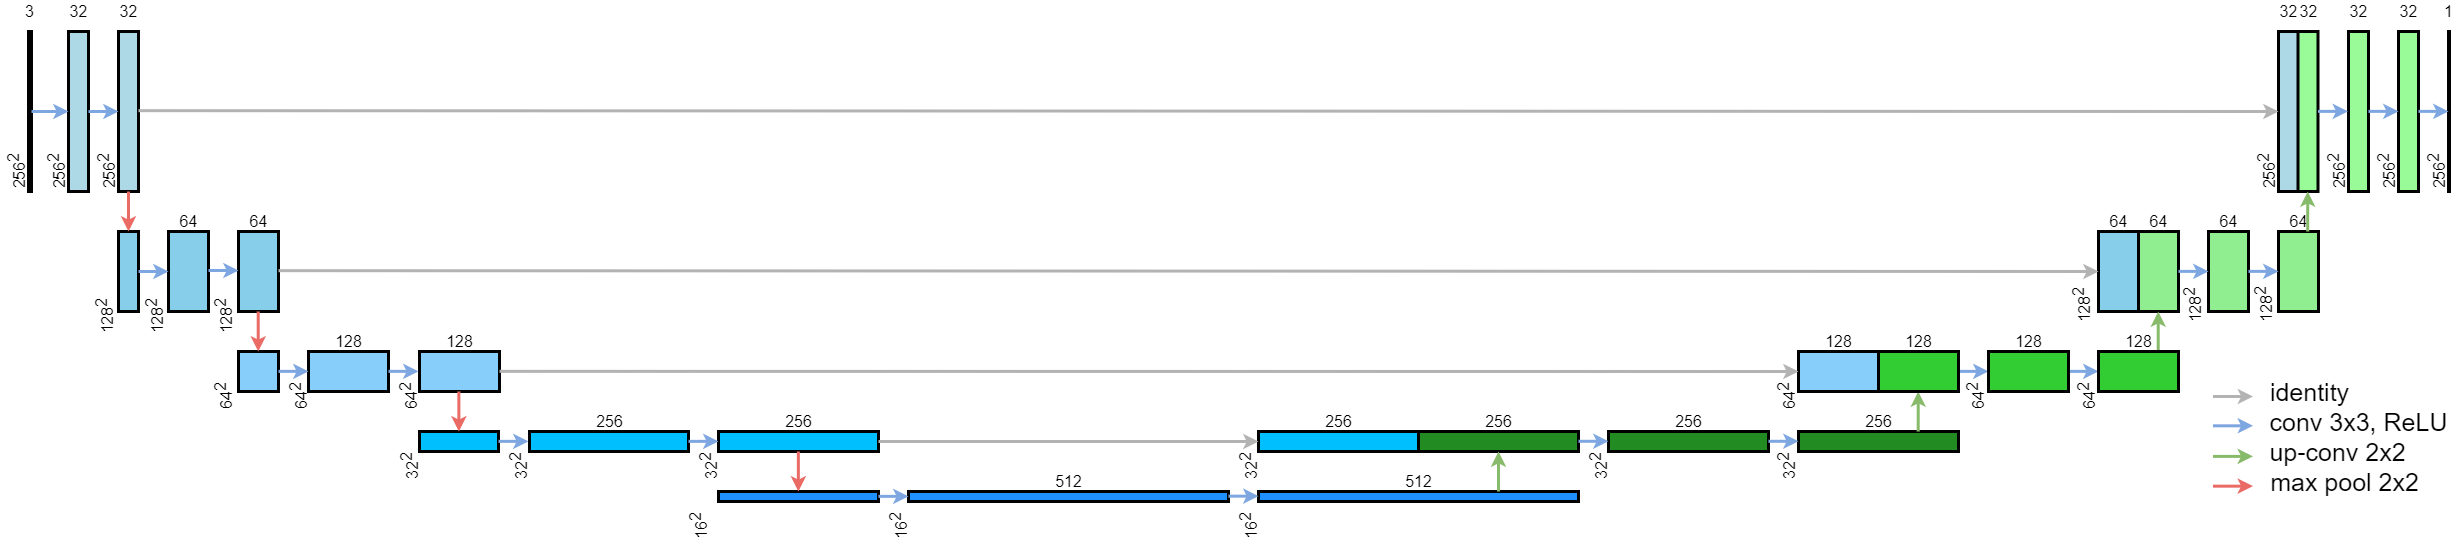
\includegraphics[width=\linewidth]{img/model_UNet.png}
  \caption{Model architecture of UNet}
  \label{fig:unet}
\end{figure*}

\begin{figure*}[t]
  \centering
  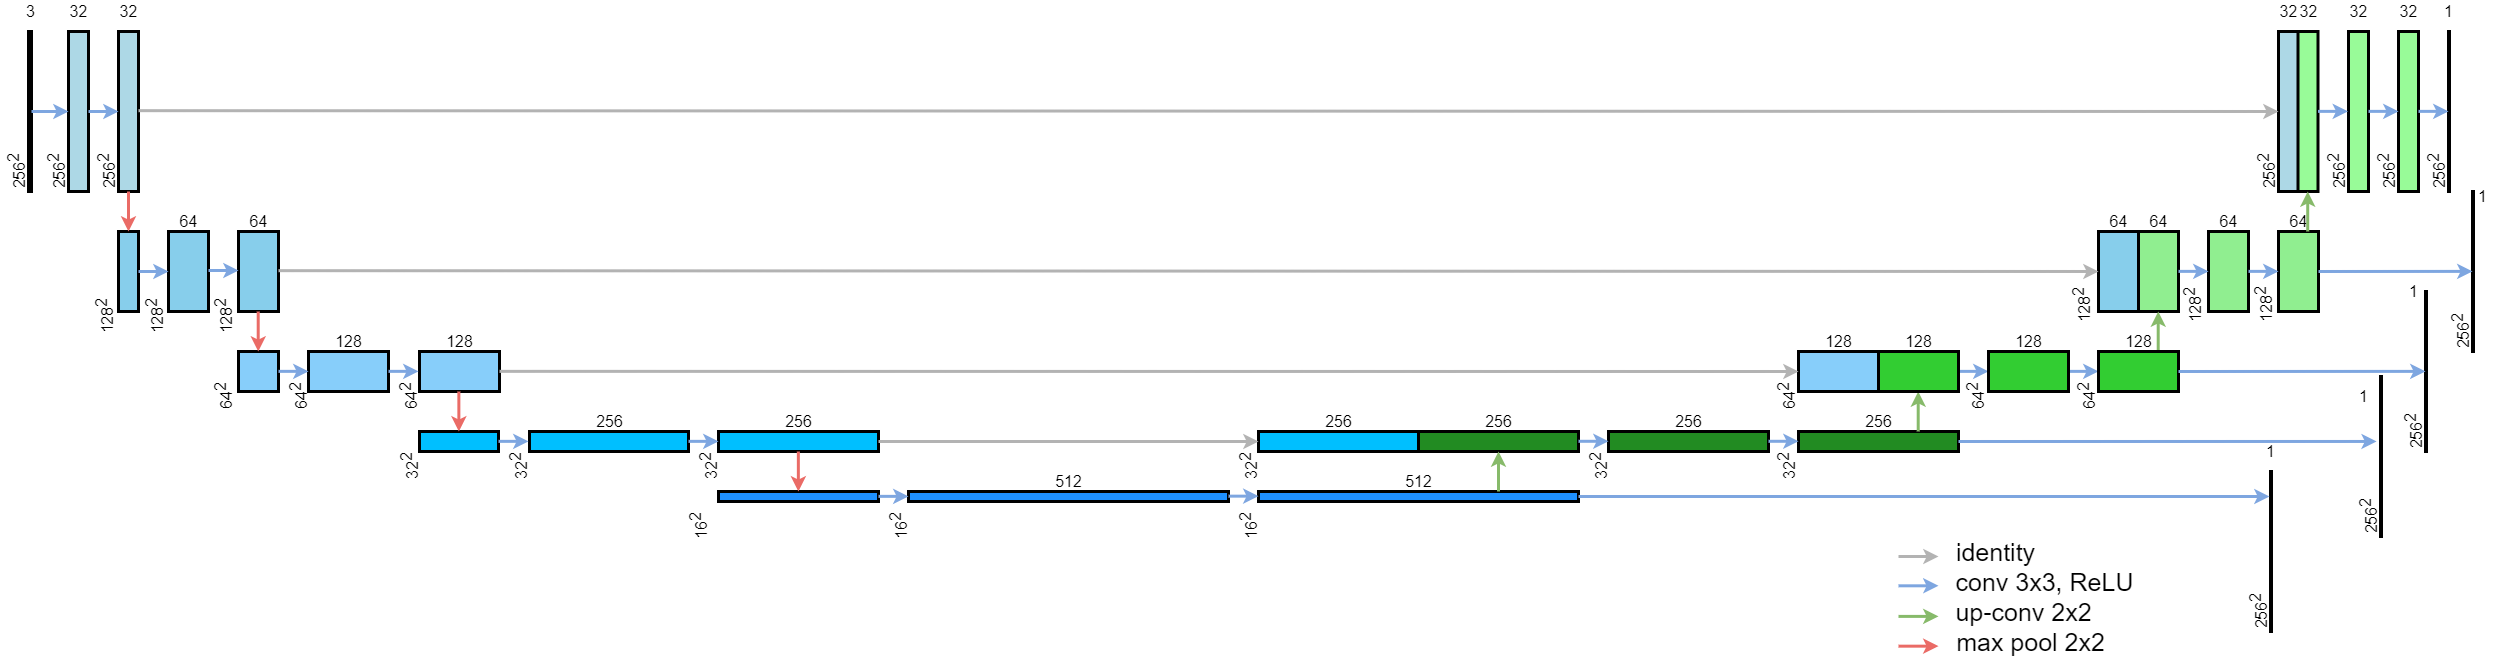
\includegraphics[width=\linewidth]{img/model_MultiUNet.png}
  \caption{Model architecture of Multi-Output UNet}
  \label{fig:multiOutUnet}
\end{figure*}

\subsection{Model Architecture}

\subsubsection{UNet}
For image segmentation, especially medical image \linebreak segmentation, UNet\cite{ronnebergerUNet} is one of the most successful methods. 
This method was proposed at the 2015 MICCAI conference, and there are already more than 14000 references.
The architecture of UNet is shown in Fig.~\ref{fig:unet}.
U-shaped structure and skip-connection are two very important features of UNet.
Through convolution and max pooling layer, the image will be sampled 4 times, and the batch size is 2.
Correspondingly, the high-level semantic feature will be restored to the resolution of the original picture through the up-sampling layer.
Because of the U-shaped structure, the feature map incorporates more high-level features.
The skip connection is used in each level of UNet, which ensures the low-level features in the feature map.
In Fig.~\ref{fig:unet}, each block represents the result of a convolution unit. 
The resolution of each block is displayed on the left, and the number of layers is displayed on the top.
The image as input has 3 layers for three color channels, while the output has only one binary layer, representing blood or non-blood.
The blue arrows indicate the convolution units, which is composed of a 2D convolution and a ReLU filter.
The kernel size of 2D convolutions is {$3 \times 3$}.
In order to find the suitable learning rate for UNet, this model has been trained many times with different learning rates. 
The decreasing loss curve for each learning rate is shown in Fig.~\ref{fig:unetLearningRate}.
\par
The smaller the learning rate, the smaller the oscillation of the training curve, but it will take more time to reach the convergence state.
To finish the training process with 100 epoch and 5-ford cross validation, it takes already sbout 24 hours.
As a compromise, 0.0001 is the suitable learning rate for UNet and will be used for all models.

\begin{figure}[h]
  \centering
  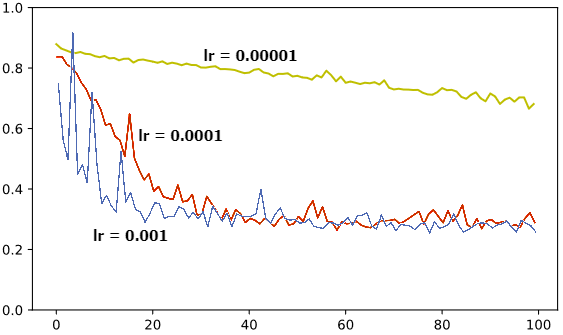
\includegraphics[width=\linewidth]{img/learning_rate.png}
  \caption{Loss curve with different \\ learning rate}
  \label{fig:unetLearningRate}
\end{figure}

\subsubsection{Multi-Output UNet}
Multi-Output UNet is a transformation of UNet. 
It will create five images from five different depths.
Losses will be calculated separately using the same ground truth mask, and the weighted sum of all calculated losses is the final loss.
In ordinary UNet, features from deeper layer will be compressed many times by convolution. 
And the output focus only on the result from lowest layer.
By calculating the weighted sum of losses, Multi-Output UNet treats the convolution results of each depth fairly.
The purpose is to make the estimation contain more general information and ignoring details.
The architecture is shown in Fig.~\ref{fig:multiOutUnet}.
\par
In implementation, the learning rate used is also 0.0001, and each cross-validation is trained 100 epochs.
The same weight is given to all five images whensumming up losses, so the equation is defined as:
\begin{equation} Loss_{sum}(I_m, \{I_i|i\in [0, 4]\}) = \frac{\sum_{i\in [0, 4]}loss(I_m, I_i)}{5}  \end{equation}

\subsubsection{ResNet}
The proposition of the deep residual network(ResNet)\cite{hekaimingResNet} is a milestone in the history of CNN images.
It have emerged as a family of extremely deep architectures showing \linebreak compelling accuracy and nice convergence behaviors. 
The involved models in this project are FCN\_ResNet50\cite{longResNet} and DeepLabV3\_ResNet50\cite{chenResNet} from torchvision.
Both models are used in not-pretrained model and with 2 as num\_classes.
The output of ResNet are the posibility that one pixel \linebreak belongs to those classes. 
With the argmax function \linebreak afterwords, the estimated class can be found. 
So the classes number in the output of ResNet should be 2 instead of 1.
\par
There are also a special requirment, that the imput \linebreak image should be normalized to [0.485, 0.456, 0.406] as mean value for three color channel and [0.229, 0.224, 0.225] as standard deviation.
Those normalisation are done by using Normalize() function from torch vision.

\section{Results}

\subsection{UNet}
The evaluation result for UNet after 100 epochs are shown in TABLE~\ref{tab:UNetResult} and the evaluation curve in Fig.~\ref{fig:UNetTrainingCurve}
Some estimation examples are shown in Fig.~\ref{fig:UNetEsti}.
\par
In Fig.~\ref{fig:UNetEsti}, green line represents ground truth area and yellow line shows estimation.

\begin{table}[ht]
  \begin{tabularx}{\linewidth}{@{}l*{10}{C}c@{}}
    \toprule
      { }             & loss     & precision  & recall  & specificity & {$f_1$}   \\ 
    \midrule
      cross\_val 1    & 0.1865   & 0.8739     & 0.7618  & 0.9896      &  0.8135   \\
      cross\_val 2    & 0.3727   & 0.7479     & 0.5571  & 0.9848      &  0.6273   \\
      cross\_val 3    & 0.3065   & 0.8558     & 0.5912  & 0.9956      &  0.6935   \\
      cross\_val 4    & 0.1958   & 0.7421     & 0.8942  & 0.9672      &  0.8042   \\
      cross\_val 5    & 0.2897   & 0.7781     & 0.6560  & 0.9918      &  0.7103   \\ 
    \addlinespace
      average         & 0.2702   & 0.7996     & 0.6920  & 0.9858      &  0.7298   \\ 
    \bottomrule
  \end{tabularx}
  \caption{Evaluation of UNet}
  \label{tab:UNetResult}
\end{table}

\begin{figure}[h]
  \centering
  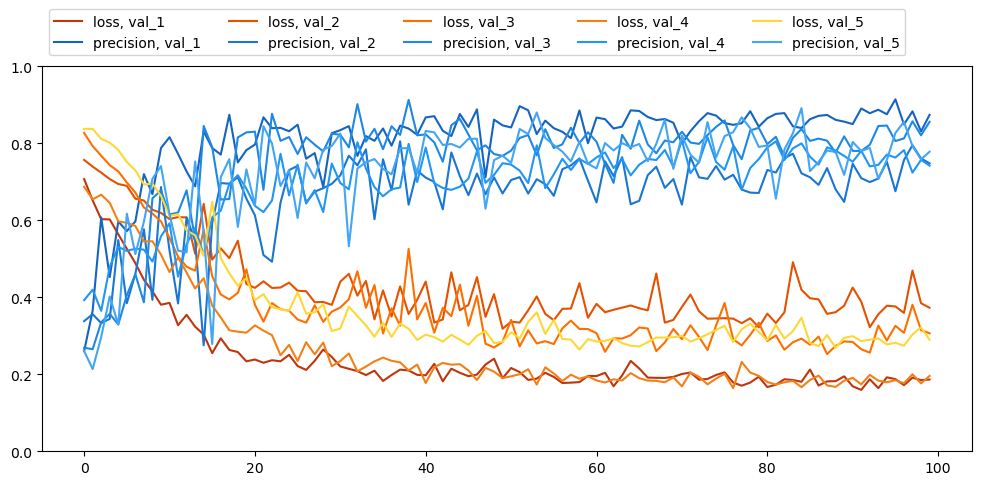
\includegraphics[width=\linewidth]{img/trainingCurve_UNet.png}
  \caption{Evaluation curve of UNet}
  \label{fig:UNetTrainingCurve}
\end{figure}

\begin{figure}[h]
  \centering
  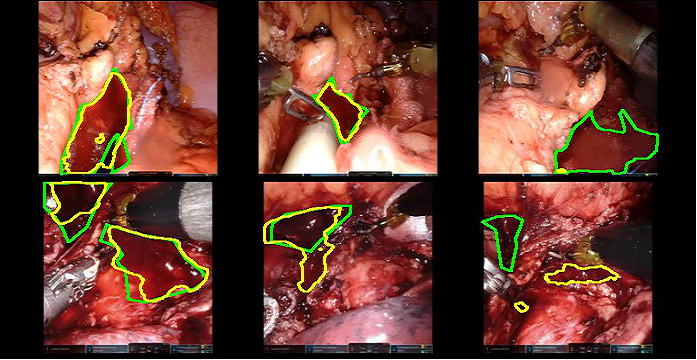
\includegraphics[width=\linewidth]{img/Estimation_output_UNet.png}
  \caption{Segmentation (as yellow) of UNet}
  \label{fig:UNetEsti}
\end{figure}

\subsection{Multi-Output UNet}
The evaluation result for Multi-Output UNet after 100 epochs are shown in TABLE~\ref{MultiOutUNetResult} and the evaluation curve in Fig.~\ref{fig:MultiOutUNetTrainingCurve}
Some estimation examples are shown in Fig.~\ref{fig:MultiOutUNetEsti}.
\par
In Fig.~\ref{fig:MultiOutUNetEsti}, green line represents ground truth area and yellow line shows estimation.
\begin{table}[ht]
  \begin{tabularx}{\linewidth}{@{}l*{10}{C}c@{}}
    \toprule
      { }             & loss      & precision   & recall  & specificity & {$f_1$}   \\ 
    \midrule
      cross\_val 1    & 0.1806    & 0.8042      & 0.8409  & 0.9782      & 0.8194    \\
      cross\_val 2    & 0.3637    & 0.7276      & 0.5727  & 0.9824      & 0.6363    \\
      cross\_val 3    & 0.3284    & 0.8490      & 0.5691  & 0.9954      & 0.6716    \\
      cross\_val 4    & 0.2144    & 0.7159      & 0.8763  & 0.9644      & 0.7856    \\
      cross\_val 5    & 0.3107    & 0.8441      & 0.5859  & 0.9955      & 0.6892    \\
    \addlinespace
      average         & 0.2796    & 0.7882      & 0.6890  & 0.9832      & 0.7204    \\ 
    \bottomrule
  \end{tabularx}
  \caption{Evaluation of Multi-Output UNet}
  \label{MultiOutUNetResult}
\end{table}

\begin{figure}[h]
  \centering
  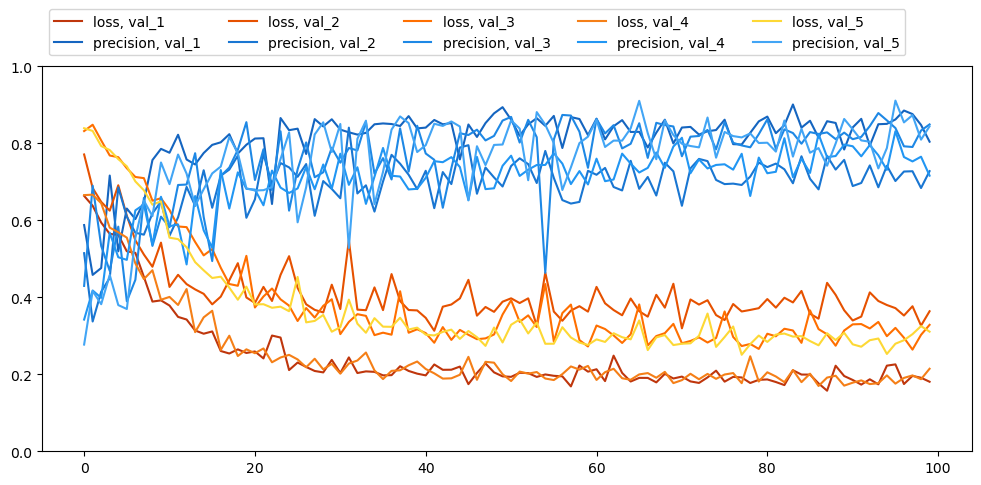
\includegraphics[width=\linewidth]{img/trainingCurve_MultiUNet.png}
  \caption{Evaluation curve of Multi-Output UNet}
  \label{fig:MultiOutUNetTrainingCurve}
\end{figure}

\begin{figure}[h]
  \centering
  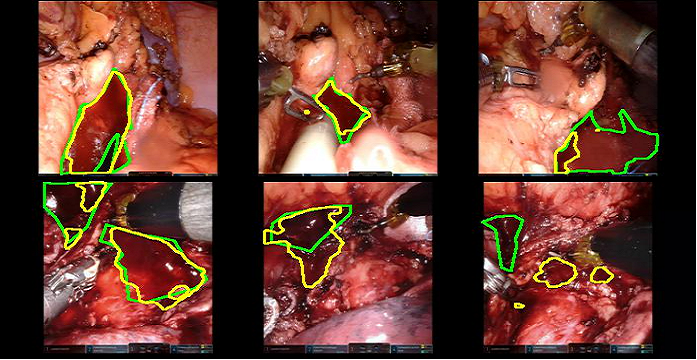
\includegraphics[width=\linewidth]{img/Estimation_output_MultiOut_UNet.png}
  \caption{Segmentation (as yellow) of Multi-Output UNet}
  \label{fig:MultiOutUNetEsti}
\end{figure}

\subsection{ResNet-based segmentation networks}
The evaluation result for ResNet after 100 epochs are shown in TABLE~\ref{tab:FCNResNet50Result} and TABLE~\ref{tab:DeepLabV3ResNet50}. 
In Fig.~\ref{fig:FCNResNet50TrainingCurve} and Fig.~\ref{fig:DeepLabTrainingCurve} are evaluation curves.
The estimation examples are shown in Fig.~\ref{fig:FCNResNet50Esti} and Fig.~\ref{fig:DeepLabEsti}.

\begin{table}[h]
  \begin{tabularx}{\linewidth}{@{}l*{10}{C}c@{}}
    \toprule
      { }             & loss    & precision   & recall  & specificity & {$f_1$} \\ 
    \midrule
      cross\_val 1    & 0.1582  & 0.9062      & 0.7875  & 0.9917      & 0.8418  \\
      cross\_val 2    & 0.3586  & 0.7570      & 0.5697  & 0.9850      & 0.6414  \\
      cross\_val 3    & 0.3576  & 0.8517      & 0.5684  & 0.9954      & 0.6424  \\
      cross\_val 4    & 0.1856  & 0.7889      & 0.8818  & 0.9745      & 0.8144  \\
      cross\_val 5    & 0.3386  & 0.7830      & 0.6201  & 0.9925      & 0.6614  \\
    \addlinespace
      average         & 0.2797  & 0.8173      & 0.6855  & 0.9878      & 0.7203  \\ 
    \bottomrule
  \end{tabularx}
  \caption{Evaluation of FCN\_ResNet50}
  \label{tab:FCNResNet50Result}
\end{table}

\begin{figure}[h]
  \centering
  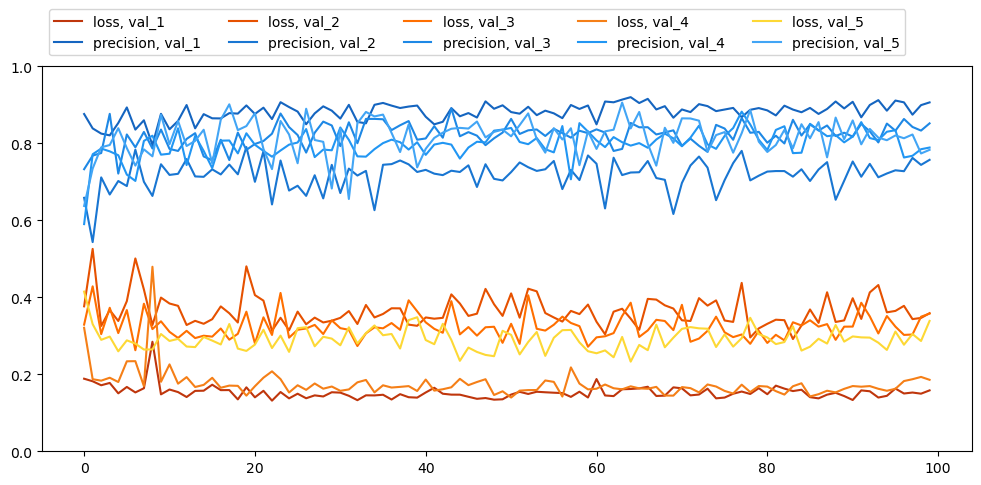
\includegraphics[width=\linewidth]{img/trainingCurve_FCN.png}
  \caption{Evaluation curve of FCN\_ResNet50}
  \label{fig:FCNResNet50TrainingCurve}
\end{figure}

\begin{figure}[h]
  \centering
  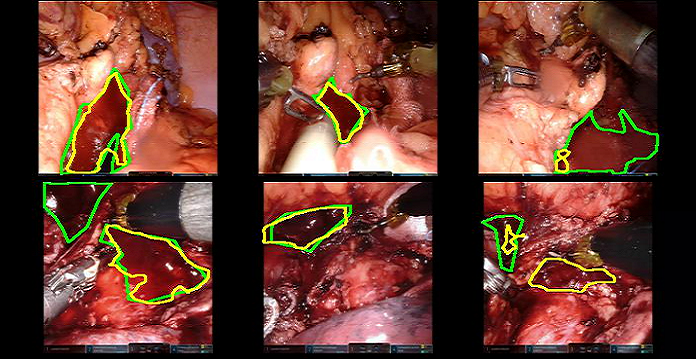
\includegraphics[width=\linewidth]{img/Estimation_output_FCN_ResNet.png}
  \caption{Segmentation (as yellow) of FCN\_ResNet50}
  \label{fig:FCNResNet50Esti}
\end{figure}

\begin{table}[t]
  \begin{tabularx}{\linewidth}{@{}l*{10}{C}c@{}}
    \toprule
      { }             & loss      & precision   & recall  & specificity & {$f_1$} \\ 
    \midrule
      cross\_val 1    & 0.1395    & 0.8891      & 0.8406  & 0.9892      & 0.8605  \\
      cross\_val 2    & 0.3478    & 0.6894      & 0.6597  & 0.9754      & 0.6522  \\
      cross\_val 3    & 0.2772    & 0.8508      & 0.6857  & 0.9942      & 0.7228  \\
      cross\_val 4    & 0.1630    & 0.8296      & 0.8807  & 0.9811      & 0.8370  \\
      cross\_val 5    & 0.2662    & 0.8358      & 0.6541  & 0.9939      & 0.7338  \\
    \addlinespace
      average         & 0.2387    & 0.8189      & 0.7442  & 0.9868      & 0.7613  \\ 
    \bottomrule
  \end{tabularx}
  \caption{Evaluation of DeepLabV3\_ResNet50}
  \label{tab:DeepLabV3ResNet50}
\end{table}

\begin{figure}[h]
  \centering
  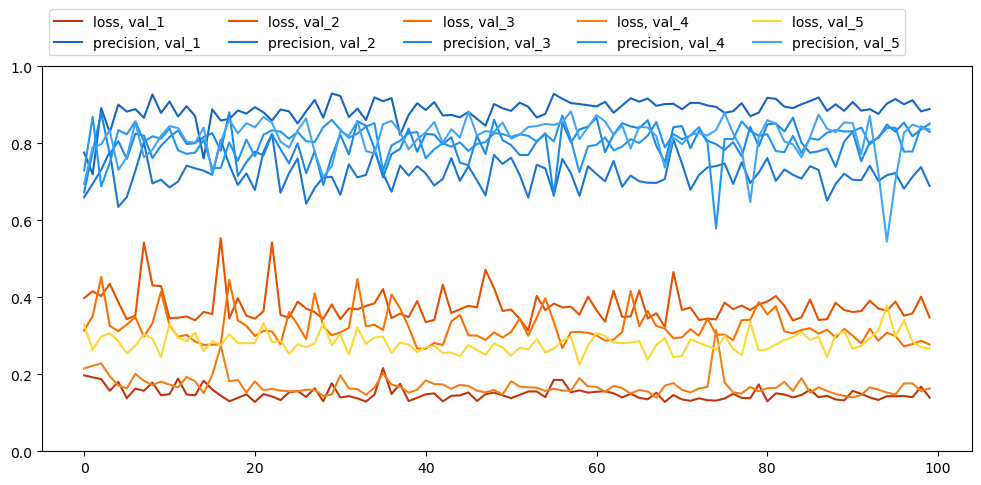
\includegraphics[width=\linewidth]{img/trainingCurve_Deeplab.png}
  \caption{Evaluation curve of DeepLabV3\_ResNet50}
  \label{fig:DeepLabTrainingCurve}
\end{figure}

\begin{figure}[t]
  \centering
  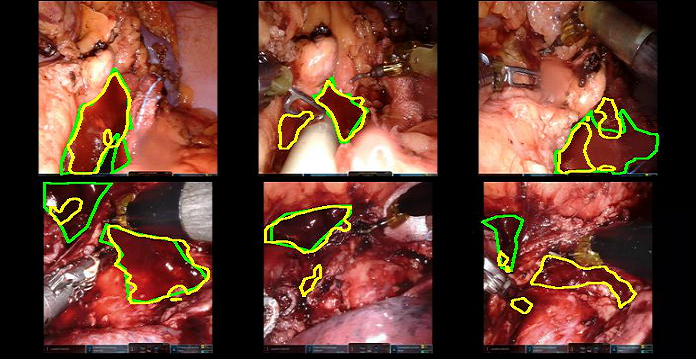
\includegraphics[width=\linewidth]{img/Estimation_output_Deeplab_ResNet}
  \caption{Segmentation (as yellow) of DeepLabV3\_ResNet50}
  \label{fig:DeepLabEsti}
\end{figure}

\subsection{Response time}
The response time of segmentation using different models are shown in TABLE~\ref{tab:responseTime} below:
\begin{table}[h]
  \begin{tabularx}{\linewidth}{@{}l*{10}{C}c@{}}
    \toprule
      {Response time(ms) }  & CPU                 & GPU                         \\ 
      {}                    & (i7-6700k)          & (GeForce RTX 2070)          \\ 
    \midrule
      UNet                  & 110                 & 2.5                         \\
      Multi-Output UNet     & 110                 & 2.8                         \\
      FCN\_ResNet50         & 270                 & 5.8                         \\
      DeepLabV3\_ResNet50   & 440                 & 6.2                         \\
    \bottomrule
  \end{tabularx}
  \caption{Response time of image segmentation}
  \label{tab:responseTime}
\end{table}

\section{Discussion}
As can be seen from the tables, under a learning rate of 0.0001 and 100 epochs, the four models are not particularly different.
DeepLab ResNet has the lowest average loss of 0.2387, while the average loss of other models is about 0.27.
The prediction results of the ResNet model of FCN and Deeplab are 0.8173 and 0.8189. 
However, the precision of UNet and Multi-Output UNet are 0.7996 and 0.7882 \linebreak respectively.
Although it can be seen from the data that ResNet is better than UNet, the difference between the two is not significant.
The training process of each model is shown in its line chart.
After 20 epochs, the two ResNets have reached a convergent area but UNets need more than 40.
One possible reason for this result is that ResNet has more convolutional layers. 
This can also be seen from the model parameter file saved at the end of training: the average size of the UNet parameter file is about 30MB, while ResNet need more than 120MB.
Due to the difference in the number of model parameters, the response time when using the model to create predictions also varies greatly.
Normal video has 60 frames per second, so in order to achieve \linebreak real-time image recognition, the processing time of each frame needs to be less than 16.6 milliseconds.
\par
From TABLE~\ref{tab:responseTime}, it is easy to see that real-time \linebreak segmentation requires the help of GPU.
The \linebreak experiments were done using ASUS GeForce RTX 2070 and the response time of segmentation with ResNet and UNet were 7 and 3.5 milliseconds, respectively.
In addition to image segmentation, the program also needs to complete the preprocessing of the image, the conversion of the data format between the CPU and GPU and the final display in 16.6 milliseconds.
From this point of view, UNet has the better chance to be real-time.


% An example of a floating figure using the graphicx package.
% Note that \label must occur AFTER (or within) \caption.
% For figures, \caption should occur after the \includegraphics.
% Note that IEEEtran v1.7 and later has special internal code that
% is designed to preserve the operation of \label within \caption
% even when the captionsoff option is in effect. However, because
% of issues like this, it may be the safest practice to put all your
% \label just after \caption rather than within \caption{}.
%
% Reminder: the "draftcls" or "draftclsnofoot", not "draft", class
% option should be used if it is desired that the figures are to be
% displayed while in draft mode.
%
%\begin{figure}[!t]
%\centering
%\includegraphics[width=2.5in]{myfigure}
% where an .eps filename suffix will be assumed under latex, 
% and a .pdf suffix will be assumed for pdflatex; or what has been declared
% via \DeclareGraphicsExtensions.
%\caption{Simulation results for the network.}
%\label{fig_sim}
%\end{figure}

% Note that the IEEE typically puts floats only at the top, even when this
% results in a large percentage of a column being occupied by floats.
% However, the Computer Society has been known to put floats at the bottom.


% An example of a double column floating figure using two subfigures.
% (The subfig.sty package must be loaded for this to work.)
% The subfigure \label commands are set within each subfloat command,
% and the \label for the overall figure must come after \caption.
% \hfil is used as a separator to get equal spacing.
% Watch out that the combined width of all the subfigures on a 
% line do not exceed the text width or a line break will occur.
%
%\begin{figure*}[!t]
%\centering
%\subfloat[Case I]{\includegraphics[width=2.5in]{box}%
%\label{fig_first_case}}
%\hfil
%\subfloat[Case II]{\includegraphics[width=2.5in]{box}%
%\label{fig_second_case}}
%\caption{Simulation results for the network.}
%\label{fig_sim}
%\end{figure*}
%
% Note that often IEEE papers with subfigures do not employ subfigure
% captions (using the optional argument to \subfloat[]), but instead will
% reference/describe all of them (a), (b), etc., within the main caption.
% Be aware that for subfig.sty to generate the (a), (b), etc., subfigure
% labels, the optional argument to \subfloat must be present. If a
% subcaption is not desired, just leave its contents blank,
% e.g., \subfloat[].


% An example of a floating table. Note that, for IEEE style tables, the
% \caption command should come BEFORE the table and, given that table
% captions serve much like titles, are usually capitalized except for words
% such as a, an, and, as, at, but, by, for, in, nor, of, on, or, the, to
% and up, which are usually not capitalized unless they are the first or
% last word of the caption. Table text will default to \footnotesize as
% the IEEE normally uses this smaller font for tables.
% The \label must come after \caption as always.
%
%\begin{table}[!t]
%% increase table row spacing, adjust to taste
%\renewcommand{\arraystretch}{1.3}
% if using array.sty, it might be a good idea to tweak the value of
% \extrarowheight as needed to properly center the text within the cells
%\caption{An Example of a Table}
%\label{table_example}
%\centering
%% Some packages, such as MDW tools, offer better commands for making tables
%% than the plain LaTeX2e tabular which is used here.
%\begin{tabular}{|c||c|}
%\hline
%One & Two\\
%\hline
%Three & Four\\
%\hline
%\end{tabular}
%\end{table}


% Note that the IEEE does not put floats in the very first column
% - or typically anywhere on the first page for that matter. Also,
% in-text middle ("here") positioning is typically not used, but it
% is allowed and encouraged for Computer Society conferences (but
% not Computer Society journals). Most IEEE journals/conferences use
% top floats exclusively. 
% Note that, LaTeX2e, unlike IEEE journals/conferences, places
% footnotes above bottom floats. This can be corrected via the
% \fnbelowfloat command of the stfloats package.


\section{Conclusion}
The first contribuition of this project is, that a new dataset of surgery images is created.
There are four convolutional \linebreak neural network models involved in this project: UNet, Multi-Output UNet, FCN\_ResNet50 and DeepLabV3\_ResNet50.
Then the models are realized and all estimations are acceptable. 
The dice loss is used as loss function.
The four models are also compared using loss, accuracy, recall and other parameters calculated from the confusion matrix.
As a conclusion, the difference of accuracy between UNet and ResNet is very small. The response time of UNet is shorter than FCN\_ResNet50 and DeepLabV3\_ResNet50, which is important for real-time segmentation.
The manual annotation of this dataset took a long time. 
A new method to annotate the blood area and the corresponding new loss function should be future work.


% if have a single appendix:
%\appendix[Proof of the Zonklar Equations]
% or
%\appendix  % for no appendix heading
% do not use \section anymore after \appendix, only \section*
% is possibly needed

% use appendices with more than one appendix
% then use \section to start each appendix
% you must declare a \section before using any
% \subsection or using \label (\appendices by itself
% starts a section numbered zero.)
%


% Can use something like this to put references on a page
% by themselves when using endfloat and the captionsoff option.
\ifCLASSOPTIONcaptionsoff
  \newpage
\fi


% trigger a \newpage just before the given reference
% number - used to balance the columns on the last page
% adjust value as needed - may need to be readjusted if
% the document is modified later
%\IEEEtriggeratref{8}
% The "triggered" command can be changed if desired:
%\IEEEtriggercmd{\enlargethispage{-5in}}

% references section

% can use a bibliography generated by BibTeX as a .bbl file
% BibTeX documentation can be easily obtained at:
% http://mirror.ctan.org/biblio/bibtex/contrib/doc/
% The IEEEtran BibTeX style support page is at:
% http://www.michaelshell.org/tex/ieeetran/bibtex/
%\bibliographystyle{IEEEtran}
% argument is your BibTeX string definitions and bibliography database(s)
%\bibliography{IEEEabrv,../bib/paper}
%
% <OR> manually copy in the resultant .bbl file
% set second argument of \begin to the number of references
% (used to reserve space for the reference number labels box)
\begin{thebibliography}{99}

\bibitem{cherietThresholding}Cheriet, Mohamed, Joseph N. Said, and Ching Y. Suen. "A recursive thresholding technique for image segmentation." IEEE transactions on image processing 7.6 (1998): 918-921.

\bibitem{colemanClustering}Coleman, Guy Barrett, and Harry C. Andrews. "Image segmentation by clustering." Proceedings of the IEEE 67.5 (1979): 773-785.

\bibitem{tobiasHistogramThresholding}Tobias, Orlando José, and Rui Seara. "Image segmentation by histogram thresholding using fuzzy sets." IEEE transactions on Image Processing 11.12 (2002): 1457-1465.


\bibitem{ronnebergerUNet}Ronneberger O., Fischer P., Brox T. (2015) U-Net: Convolutional Networks for Biomedical Image Segmentation. In: Navab N., Hornegger J., Wells W., Frangi A. (eds) Medical Image Computing and Computer-Assisted Intervention – MICCAI 2015. MICCAI 2015. Lecture Notes in Computer Science, vol 9351. Springer, Cham

\bibitem{longResNet}Long, Jonathan, Evan Shelhamer, and Trevor Darrell. "Fully convolutional networks for semantic segmentation." Proceedings of the IEEE conference on computer vision and pattern recognition. 2015.

\bibitem{chenResNet}Chen, Liang-Chieh, et al. "Rethinking atrous convolution for semantic image segmentation." arXiv preprint arXiv:1706.05587 (2017).

\bibitem{sunMultiOutUNet}Sun, Tao, et al. "Stacked U-Nets With Multi-Output for Road Extraction." CVPR Workshops. 2018.

\bibitem{diceloss}Drozdzal, Michal, et al. "The importance of skip connections in biomedical image segmentation." Deep Learning and Data Labeling for Medical Applications. Springer, Cham, 2016. 179-187.
\bibitem{hekaimingResNet}He, Kaiming, Xiangyu Zhang, Shaoqing Ren, and Jian Sun. "Identity mappings in deep residual networks." In European conference on computer vision, pp. 630-645. Springer, Cham, 2016.
\end{thebibliography}

% biography section
% 
% If you have an EPS/PDF photo (graphicx package needed) extra braces are
% needed around the contents of the optional argument to biography to prevent
% the LaTeX parser from getting confused when it sees the complicated
% \includegraphics command within an optional argument. (You could create
% your own custom macro containing the \includegraphics command to make things
% simpler here.)
%\begin{IEEEbiography}[{\includegraphics[width=1in,height=1.25in,clip,keepaspectratio]{mshell}}]{Michael Shell}
% or if you just want to reserve a space for a photo:

% You can push biographies down or up by placing
% a \vfill before or after them. The appropriate
% use of \vfill depends on what kind of text is
% on the last page and whether or not the columns
% are being equalized.

%\vfill

% Can be used to pull up biographies so that the bottom of the last one
% is flush with the other column.
%\enlargethispage{-5in}



% that's all folks
\end{document}


